%!TEX root = /Users/dedan/bccn/lab_rotations/johannes/report/report.tex
\chapter{Results} % (fold)
\label{sg:cha:results}

This work showed that it is possible to use the concept of \emph{proto-objects} also in computer vision. The approach led to a realtime object-recognition system which uses the available computational resources much more efficiently as the expensive computation of SIFT-features is only applied to small patches of the original image. This allows for the analysis of almost 30 frames/s. Another advantage of the proto-object approach is that the image patch that contains the object can be masked to reduce the amount of SIFT-features wrongly assigned to an object and therefore minimizes false-positive matches against the database of objects. Furthermore the available depth information in combination with the keypoint scale could be used to rule out false-positive matches in the database (see end of section \ref{sg:sec:sift}).

\begin{table}[ht]
    \centering
    \begin{tabular}{cc}
    \hline
    SIFT only in patches & 26,5\\
    \hline
    SIFT on whole image & 322\\
    \hline
    \end{tabular}
    \caption{average computation time [ms] over 500 frames}
\end{table}
\begin{figure}[ht]
    \centering
        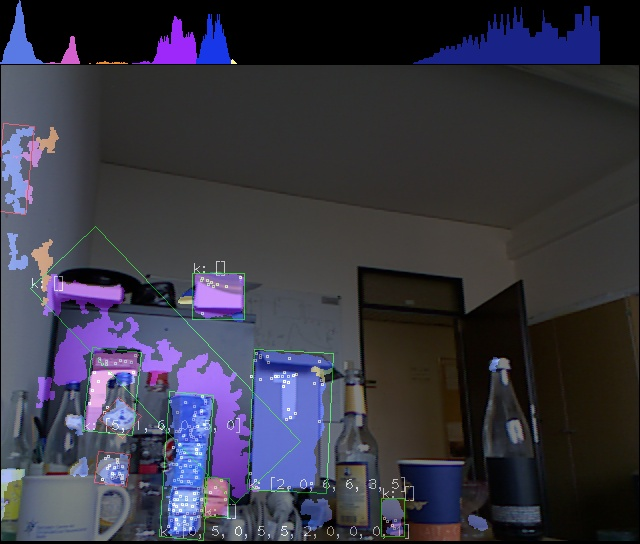
\includegraphics[width=0.4\textwidth]{images/benchmark.jpg}
    \caption{This image was used for the SIFT-feature computation time benchmark}
    \label{sg:fig:images_benchmark}
\end{figure}

Unfortunately there was very limited time for this project. Therefore it resulted only in a very simple implementation which nevertheless proved that it is possible to apply a very simple heuristics for the detection of proto-objects and maybe more important, it inspired many ideas of how to improve the current solution which provide a solid base for a follow-up project.

\section{Suggestions for improving the current implementation} % (fold)
\label{sg:sec:suggestions_for_improving_the_current_implementation}
\paragraph{average over time} % (fold)
\label{par:average_over_time}
The depth information has a quite high noise level and therefore the histogram clustering flickers and changes from frame to frame. As long as the scene in front of the camera does not change very rapidly the last N frames from the depth sensor could be averaged. Or maybe better only the histograms from the last N frames. I suggest to use a discount rate for the averaging to emphasize the importance of more current information.
% paragraph average_over_time (end)

\paragraph{advanced object tracking} % (fold)
\label{par:advanced_object_tracking}
The current object tracking approach (overlap of minimum bounding rectangles) is very simple and probably works only for slowly moving objects. It would also loose track of objects if they are temporarily occluded. To avoid this problems more sophisticated tracking mechanisms (e.g. Kalman filter) could be implemented
% paragraph advanced_object_tracking (end)

\paragraph{multiprocess instead of multithread} % (fold)
\label{par:multiprocess_instead_of_multithread}
Due to the global interpreter lock (GIL) there is a python inherent problem with multithreading. Currently the heavy computation (SIFT-features) is done in separated threads. Because the SIFT-features computation is done in a compiled C-program the GIL can be avoided and therefore some of the power of multithreading can be used. However the used SIFT library (which normally uses all available cores of the computer) uses only one core per thread. This can possibly be avoided when processes are used instead of threads, it is just a bit more complicated to implement as sharing memory is more difficult between processes than in between threads.
% paragraph multiprocess_instead_of_multithread (end)

\paragraph{improved scheduler} % (fold)
\label{par:improved_scheduler}
Keypoints are only computed on objects which have been seen over at least N frames and when computational resources are available. Objects are also periodically rescheduled to account for changes in the features (e.g. due to rotation). A more sophisticated scheduler with priority classes could be implemented according to the following ideas:
\begin{description}
    \item[class 1] new (not yet sifted) objects have highest priority
    \item[class 2] recompute SIFT-features whenever the computational resources are available
    \item[class 2] objects within class 2 could be ordered by size, distance, saliency, etc..
    \item[class 3] what was already sifted but nothing found stays in the list (because of possible rotation, etc) but with lowest priority class
\end{description}
% paragraph improved_scheduler (end)

\paragraph{high resolution images} % (fold)
\label{par:high_resolution_images}
The Kinect camera can give high-resolution images (1280x1024) on a lower rate of 15 Hz. In a scene without too rapid changes it could be useful to take a high-resolution image once in a while and to compute the sift features on this image. 
% paragraph high_resolution_images (end)

\paragraph{Color histogram mapping} % (fold)
\label{par:color_histogram_mapping}
In object recognition there are many approaches of using the color-histogram to detect objects. But usually it is a big problem that the shape and border of the objects is not available. The proto-object approach allows to computer global features like the color histogram in the preselected area. This color histogram could then be used either as a first rough match against the database of objects to rule out objects which don't match the color at all or as a complete alternative to the computation of SIFT-features.
% paragraph color_histogram_mapping (end)

\paragraph{Iterative histogram clustering} % (fold)
\label{par:iterative_histogram_clustering}
The current histogram approach has a problem with objects that spread over several \emph{hills} of the histogram. These objects are segmented and later on falsely detected as several objects. To avoid this problem the histogram clustering algorithm could be extended to regard neighborhood relations of pixels when separating the \emph{hills}.
% paragraph iterative_histogram_clustering (end)

% section suggestions_for_improving_the_current_implementation (end)

% section results (end)
















